% ==================================================
% فصل ترجمه مقاله Nature
% ==================================================

\chapter*{کاهش خطای کوانتومی (خوانش)}
\label{intro}

هدف این پژوهش اعمال روش های مختلف یادگیری ماشین (کلاسیک و کوانتومی) برای کاهش خطای خوانش کیوبیت ها است. در حال حاضر تمرکز بر یک دیتاست حاصل از خوانش چهار کیوبیت در فضای کوادریچر-فاز( \lr{Q-I}) است. 
داده ها در قالب 16 فایل متنی با نام هایی از \lr{0000.txt}
تا 
\lr{1111.txt}
ارائه شده است. نام فایل ها به عنوان برچسب کلاس 
(\lr{label})
استفاده شده و هر فایل شامل چهار خط (چهار کیوبیت) و هزار مقدار مختلط برای هر خط است. 
روش های آموزش ماشین و بهبود مدل که در این جا به کار می بریم باید برای تعداد بیشتر کیوبیت قبل تعمیم باشد. چرا که کامپیوترهای کوانتمی شامل ده ها کیوبیت می شوند و روند کاهش خطا در خوانش کیوبیت ها جزء بسیار مهم در حوزه سامانه های پردازش کیوبیتی است. 
با وجود استفاده از روش‌های مختلف یادگیری ماشین کلاسیک، مهندسی ویژگی و کرنل‌های الهام‌گرفته از نگاشت‌های کوانتومی نظیر \lr{ZZ feature map}، دقت پیش‌بینی چندکلاسه در بهترین حالت به حدود ۳۸ تا ۳۹ درصد محدود شده است. 

این گزارش شامل مراحل تحلیل داده، اعمال مدل های مختلف، مهندسی داده، بررسی نتایج و در نهایت طرح پیشنهادات و راهکارهای مرتبط است. 

%============
\section*{شرح مسئله}
\label{sec:explain}

خوانش حالت کیوبیت‌ها یکی از چالش‌های اساسی در سامانه‌های محاسبات کوانتومی مبتنی بر پلتفرم‌هایی نظیر کیوبیت‌های ابررسانا یا یون‌های به‌دام‌افتاده است. در این سامانه‌ها، اطلاعات حالت کوانتومی به‌طور مستقیم قابل اندازه‌گیری نیست و از طریق فرآیندهای خوانش غیرمستقیم استخراج می‌شود. 


در بسیاری از پلتفرم‌ها (به‌ویژه کیوبیت‌های ابررسانا)، خوانش کیوبیت در \lr{dispersive regime} انجام می‌شود. در این حالت، حالت کیوبیت باعث تغییر کوچکی در فرکانس تشدیدگر می‌شود و این تغییر از طریق اندازه‌گیری سیگنال‌های \(I\) و \(Q\) (مولفه‌های درفاز و درتعامد) استخراج می‌گردد.

مهم‌ترین منابع خطای readout عبارت‌اند از:
\begin{itemize}
	\item نویز تقویت‌کننده‌ها و زنجیره‌ی اندازه‌گیری
	\item هم‌پوشانی توزیع آماری سیگنال‌های مربوط به حالت‌های \(|0\rangle\) و \(|1\rangle\)
	\item محدودیت‌های زمانی در اندازه‌گیری (\lr{trade-off} بین سرعت و دقت)
	\item برهم‌کنش ناخواسته‌ی کیوبیت‌ها در سیستم‌های چندکیوبیتی
\end{itemize}
این فرآیندهای اندازه گیری معمولاً منجر به سیگنال‌هایی در فضای کوادریچر می‌شوند که به‌صورت نقاطی در صفحه‌ی مختلط \lr{(I,Q)} نمایش داده می‌شوند.

\begin{figure}[t]
	\centering
	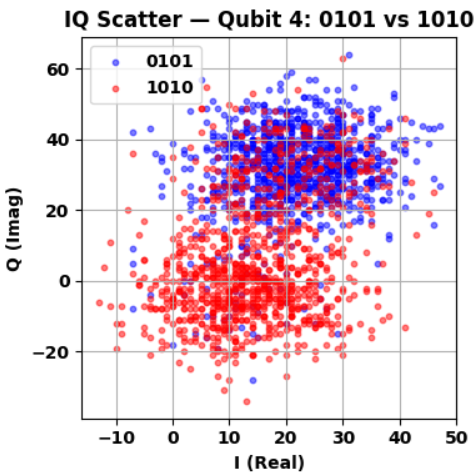
\includegraphics[width=0.75\linewidth]{figs/iq.png}
	\caption{یک نمونه از سیگنال‌های خوانش در صفحه‌ی \(I,Q\) (اندازه گیری برای کیوبیت چهارم). هم‌پوشانی توزیع آماری نقاط متناظر با حالت‌های \(|0\rangle\) و \(|1\rangle\) یکی از منابع اصلی خطای readout است.برای }
	\label{fig:IQ}
\end{figure}
در این تحقیق، داده‌های مربوط به چهار کیوبیت مورد بررسی قرار گرفته‌اند. هر نمونه‌ی داده شامل چهار عدد مختلط است که هر یک متناظر با خوانش یک کیوبیت می‌باشد. برچسب هر نمونه یکی از ۱۶ حالت ممکن$ \ket{q_4 q_3 q_2 q_1}$ است. هدف اصلی، طراحی یک مدل طبقه‌بندی است که بتواند با دریافت این چهار خوانش مختلط، حالت کامل سامانه‌ی چهار کیوبیتی را پیش‌بینی کند.


در جدول \ref*{tab:ml_readout} مقایسه ای بین روش های مدل سازی که در این پژوهش به کار رفت به صورت مختصر به صورت مقایسه ای اورده شده است. 

%====
\begin{table}[t]
	\centering
	\caption{مقایسه‌ی روش‌های متداول یادگیری ماشین برای کاهش خطای readout کیوبیت‌ها}
	\label{tab:ml_readout}
	\renewcommand{\arraystretch}{1.3}
	\begin{tabular}{|p{3cm}|p{3.2cm}|p{4.5cm}|p{3.8cm}|}
		\hline
		\textbf{روش} & \textbf{نوع الگوریتم} & \textbf{ویژگی‌های ورودی} & \textbf{مزایا و کاربردها} \\
		\hline
		Thresholding کلاسیک & تصمیم‌گیری خطی & نقطه‌ی انتهایی $I,Q$ & ساده و سریع، ولی دقت محدود در حضور نویز \\
		\hline
		Logistic Regression & یادگیری نظارت‌شده (خطی) & $I,Q$ یا ویژگی‌های استخراج‌شده & بهبود نسبت به threshold، تفسیرپذیر \\
		\hline
		SVM با کرنل غیرخطی & یادگیری نظارت‌شده & $I,Q$ یا Boxcar features & مرز تصمیم‌گیری غیرخطی، دقت بالا برای داده‌های نویزی \\
		\hline
		شبکه عصبی کم‌عمق & یادگیری عمیق & بردار ویژگی یا تایم‌تریس کوتاه & انعطاف‌پذیر، مناسب برای readout سریع \\
		\hline
		شبکه‌های زمانی (RNN / 1D-CNN) & مدل مبتنی بر زمان & کل تایم‌تریس $I(t),Q(t)$ & استخراج اطلاعات حداکثری، fidelity بالا \\
		\hline
		روش‌های تطبیقی آنلاین & یادگیری تدریجی & داده‌های به‌روز readout & مقاوم در برابر drift و تغییرات سیستم \\
		\hline
	\end{tabular}
\end{table}
%-===
%=======================
\section*{ساختار داده‌ها و تحلیل آماری اولیه}
هر مجموعه‌داده از ۱۶ فایل تشکیل شده است که هر فایل متناظر با یک حالت چهارکیوبیتی خاص می‌باشد. در هر فایل، برای هر کیوبیت ۱۰۰۰ نمونه‌ی اندازه‌گیری ثبت شده است. با ترکیب این داده‌ها، مجموعه‌داده‌ای شامل ۱۶۰۰۰ نمونه ایجاد شده است.

تحلیل‌های بصری اولیه شامل ترسیم نمودارهای پراکندگی در صفحه‌ی \lr{IQ}، هیستوگرام‌ها و توابع توزیع تجمعی انجام شد. این تحلیل‌ها نشان داد که توزیع داده‌های مربوط به حالات مختلف به‌شدت هم‌پوشان هستند. حتی با تقریب توزیع‌ها به شکل گاوسی و نمایش بیضی‌های کوواریانس، جدایش خطی یا حتی غیرخطی ساده بین کلاس‌ها امکان‌پذیر نبود (شکل \ref{fig:Gauss}). این رفتار با گزارش‌های تجربی رایج در خوانش کیوبیت‌ها هم‌خوانی دارد.

\begin{figure}[t]
	\centering
	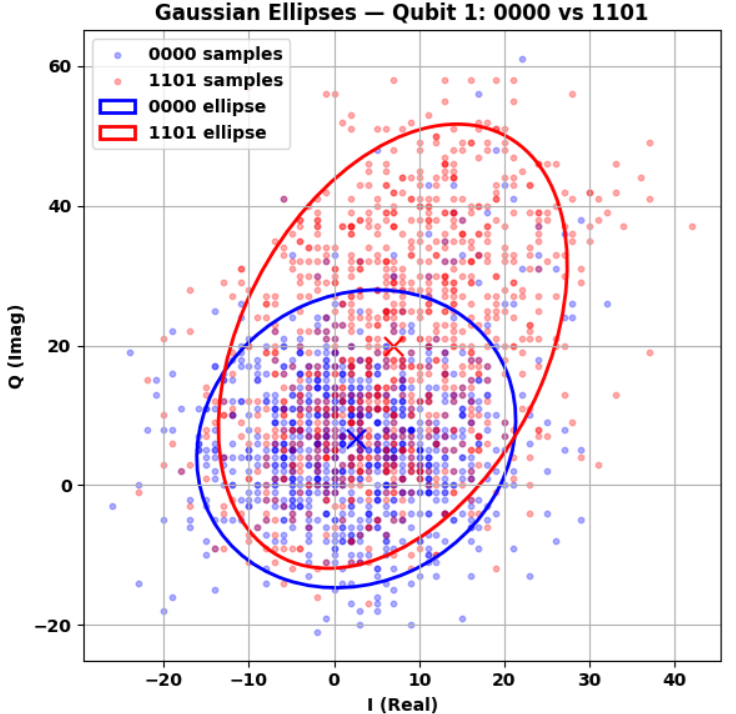
\includegraphics[width=0.85\linewidth]{figs/Gauss.png}
	\caption{تقریب توزیع بیضی های گاوسی برای  کیوبیت اول از  دو کلاس خاص (\lr{0000.txt} و \lr{1101.txt}) . همپوشی بین بیضی ها زیاد است که نشان دهنده چالش در پیش بینی کلاس ها است.}
	\label{fig:Gauss}
\end{figure}
%============================
\section*{مدل‌سازی و الگوریتم‌های یادگیری ماشین}
\textbf{مهندسی ویزگی و پیش پردازش داده ها}

در مرحله‌ی مهندسی ویژگی، دو نمایش اصلی برای داده‌های مختلط در نظر گرفته شد. در نمایش نخست، هر عدد مختلط به دو مولفه‌ی حقیقی و موهومی تجزیه شد که منجر به بردار ویژگی ۸بعدی می‌گردد. در نمایش دوم که به‌عنوان \lr{Angle Encoding} شناخته می‌شود، هر عدد مختلط به دامنه و فاز متناظر آن نگاشت شد. این نمایش از نظر فیزیکی معنادارتر بوده و به‌ویژه در ترکیب با کرنل‌های مبتنی بر توابع تناوبی مزیت دارد.

به‌منظور کاهش اثر داده‌های پرت و ناپایداری آماری، روش‌های مختلف نرمال‌سازی بررسی شدند. نتایج نشان داد که استفاده از \lr{RobustScaler} نسبت به \lr{StandardScaler} برای داده‌های نویزی آزمایشگاهی مناسب‌تر است.

در گام نخست، برای هر کیوبیت یک مدل طبقه‌بندی دودویی تنها بر اساس خوانش همان کیوبیت آموزش داده شد. 
\begin{figure}[t]
	\centering
	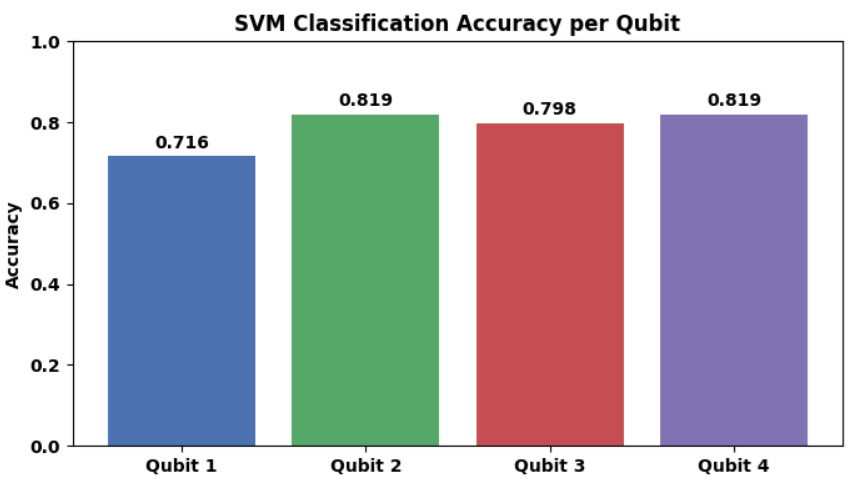
\includegraphics[width=0.95\linewidth]{figs/onebyone.png}
	\caption{مدل آموزش دو دویی تنها بر اساس خوانش تک کیوبیت.}
	\label{fig:single}
\end{figure}
دقت این مدل‌ها را می‌توان به‌عنوان سقف اطلاعاتی جدایش‌پذیری ذاتی هر کیوبیت در نظر گرفت. نتایج به‌صورت زیر به‌دست آمد:
\begin{center}
	\begin{tabular}{c c}
		\hline
		کیوبیت & دقت جدایش ذاتی \\
		\hline
		کیوبیت ۱ & \%\lr{71.3} \\
		کیوبیت ۲ & \%\lr{81.8} \\
		کیوبیت ۳ & \%\lr{80.2} \\
		کیوبیت ۴ & \%\lr{81.4} \\
		\hline
	\end{tabular}
\end{center}

این نتایج نشان می‌دهند که حتی در بهترین حالت و با استفاده از اطلاعات خوانش همان کیوبیت، خطای ذاتی قابل توجهی وجود دارد. اگر فرض شود خطاهای خوانش کیوبیت‌ها مستقل هستند، سقف دقت پیش‌بینی حالت چهارکیوبیتی را می‌توان به‌صورت تقریبی برابر حاصل‌ضرب دقت‌های تک‌کیوبیتی برآورد کرد که عددی در حدود ۳۸ درصد به‌دست می‌دهد؛
\[
71.3\% \cross 81.8\% \cross 80.2\% \cross 81.4\% \simeq 38\% 
\]
 این مقدار با بهترین دقت مشاهده‌شده در مدل چندکلاسه هم‌خوانی دارد.

\textbf{مدل های آموزش ماشین}

مدل پایه‌ی مورد استفاده، ماشین بردار پشتیبان \lr{(SVM)} بود. در ابتدا، کرنل‌های استاندارد نظیر \lr{RBF} برای طبقه‌بندی تک‌کیوبیتی و چندکلاسه مورد استفاده قرار گرفتند. در حالت تک‌کیوبیتی، دقت‌های نسبتاً بالایی برای برخی کیوبیت‌ها به‌دست آمد، اما در حالت چندکلاسه، دقت به‌طور قابل توجهی کاهش یافت.

به‌منظور لحاظ کردن هم‌بستگی‌های بین ویژگی‌ها، یک کرنل سفارشی الهام‌گرفته از \lr{ZZ feature map} معرفی شد. این کرنل شامل ترم‌های تک‌ویژگی و ترم‌های جفتی بود که به‌صورت توابع کسینوسی تعریف می‌شدند. تنظیم پارامترهای این کرنل از طریق جستجوی شبکه‌ای انجام شد. نتایج حاصل از این مدل برای کیوبیت اول در شکل \ref{fig:zz} نمایش داده شده است. 

\begin{figure}[t]
	\centering
	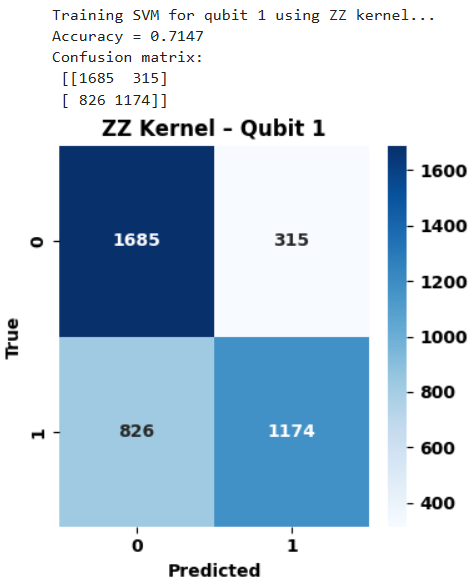
\includegraphics[width=0.6\linewidth]{figs/zz.png}
	\caption{آموزش \lr{SVM} با استفاده از کرنل کوانتمی \lr{zz feature}  برای پیش بینی کیوبیت اول.}
	\label{fig:zz}
\end{figure}

در گام دوم، وابستگی خوانش کیوبیت $i$ به حالت کیوبیت $j$ بررسی شد. برای این منظور، توزیع خوانش کیوبیت $i$ مشروط به $q_j=0$ و $q_j=1$ مقایسه گردید. معیارهایی نظیر جابه‌جایی میانگین و فاصله‌ی ماهالانوبیس بین این دو توزیع محاسبه شدند.

نتایج نشان دادند که عناصر روی قطر ماتریس وابستگی (یعنی $i=j$) به‌طور قابل توجهی بزرگ‌تر از عناصر خارج از قطر هستند، در حالی که وابستگی‌های بین‌کیوبیتی مقدار بسیار کوچکی دارند. اگرچه برخی از این وابستگی‌های ضعیف از نظر آماری معنی‌دار هستند، اما اندازه‌ی اثر آن‌ها از نظر فیزیکی ناچیز است. این موضوع نشان می‌دهد که \lr{cross-talk} بین خوانش‌ها نقش غالبی در محدودیت دقت مدل ایفا نمی‌کند.

%=================

\subsection*{تحلیل هم‌پوشانی ذاتی و وابستگی خوانش چندکیوبیتی}
به‌منظور تشخیص این‌که محدودیت دقت مدل ناشی از هم‌پوشانی ذاتی توزیع‌های خوانش است یا وابستگی و \lr{cross-talk} بین کیوبیت‌ها، یک تحلیل داده‌محور با الهام از معیارهای معرفی‌شده در مقاله‌ی
\lr{Multiplexed qubit readout quality metric beyond assignment fidelity}
انجام شد. تأکید این تحلیل بر استفاده‌ی صرف از داده‌های موجود خوانش بوده و هیچ‌گونه دسترسی به پارامترهای فیزیکی آزمایش فرض نشده است.



\subsection*{نتیجه‌گیری تحلیلی}
در این گزارش، مسئله‌ی پیش‌بینی حالت کامل چهار کیوبیت با استفاده از داده‌های خوانش کوادریچر بررسی شد. نتایج نشان می‌دهد که عامل اصلی محدودکننده‌ی دقت پیش‌بینی حالت چهارکیوبیتی، هم‌پوشانی ذاتی توزیع‌های خوانش تک‌کیوبیتی است، نه وابستگی شدید بین خوانش کیوبیت‌ها. به بیان دیگر محدودیت دقت مدل بیش از آنکه ناشی از ضعف الگوریتم‌های یادگیری ماشین باشد، ریشه در ماهیت فیزیکی فرآیند اندازه‌گیری دارد. بنابراین، افزایش قابل توجه دقت مدل تنها از طریق پیچیده‌تر کردن الگوریتم‌های یادگیری ماشین ممکن نیست و نیازمند بهبودهای فیزیکی در فرآیند خوانش و افزایش تفکیک‌پذیری اندازه‌گیری‌ها است.

%++++++++++++++++++++++